The effect of the number of training samples used for the creation of feature histograms is displayed in table \ref{tab:size_hist} and figure \ref{fig:size_hist}. The results show that the Mean Average Precision increases when more training samples per class are used. This is expected, because more training data means more patterns can be found, and thus more informative codewords can be extracted.
\begin{figure}[H]
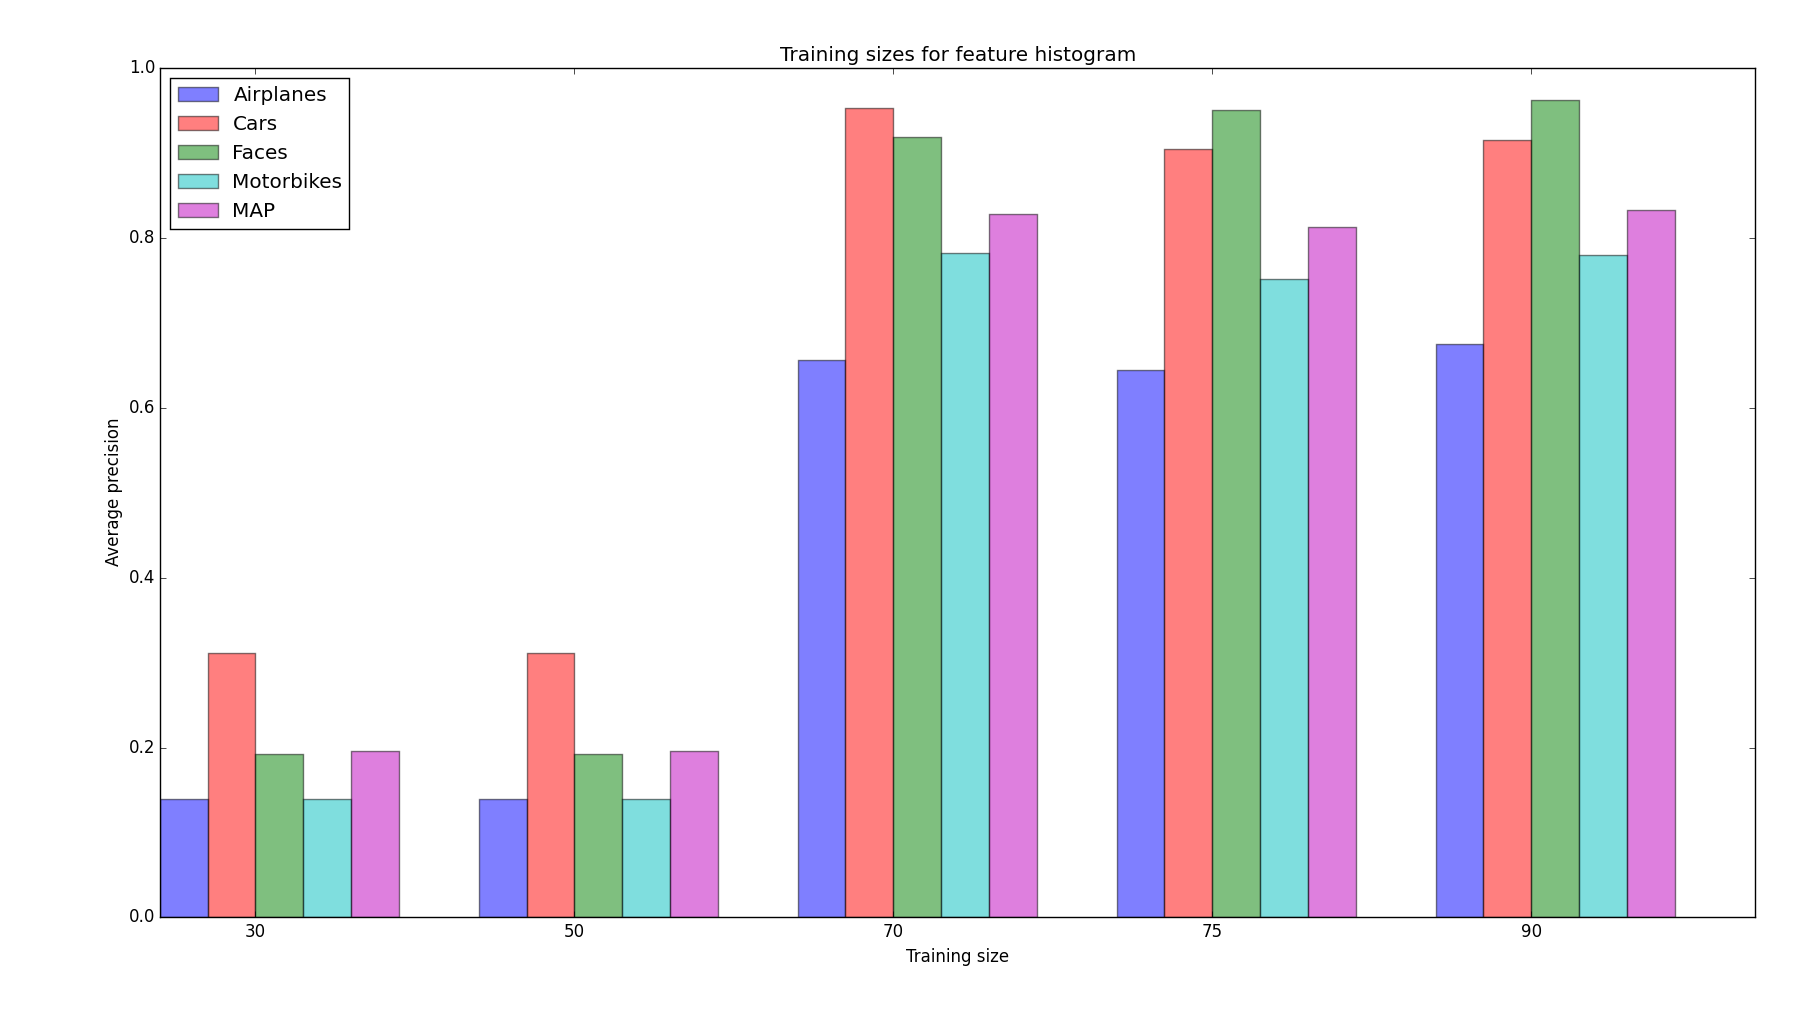
\includegraphics[width=\textwidth]{../plots/training_size_feature_histograms}
\caption{Effect of training size for histograms on AP}
\label{fig:size_hist}
\end{figure}
Figure \ref{fig:size_hist} clearly shows that MAP is highest at a training sample size of 90, with a value of 0.8334.

\begin{table}[H]
\begin{center}
\begin{tabular}{|c|ccccc|}
\hline
\textbf{Training samples} & \textbf{AP Airplanes} & \textbf{AP Cars} & \textbf{AP Faces} & \textbf{AP Motorbikes} & \textbf{MAP}\\
\hline
30 & 0.1394 & 0.3118& 0.1924& 0.1394 & 0.1958\\
50 & 0.1394 & 0.3118& 0.1924& 0.1394 & 0.1958\\
55 & 0.6516 & 0.8392 & 0.6716 & 0.7797 & 0.7355\\
60 & 0.6535 & 0.8440 & 0.9905 & 0.2919 & 0.6950\\
65 & 0.6711 & 0.9483 & 0.9440 & 0.7688 & 0.8331\\
70 & 0.6563 & 0.9534 & 0.9191 & 0.7830 & 0.8280\\
75 & 0.6447 & 0.9053 & 0.9510 & 0.7516 & 0.8132\\
90 & 0.6749 & 0.9157 & 0.9631 & 0.7798 & 0.8334\\
\hline
\end{tabular}
\caption{Effect number of training samples (per class) for feature histogram, Sift type: dense, Color space: opponent}
\label{tab:size_hist}
\end{center}
\end{table}
